%%%%%%%%%%%%%%%%%%%%%%%%%%%%%%%%%%%%%%%%%%%%%%%%%%%%%%%%%%%%%%%%%%%%%%%%%%%%%%%%%%%%
% Document data
%%%%%%%%%%%%%%%%%%%%%%%%%%%%%%%%%%%%%%%%%%%%%%%%%%%%%%%%%%%%%%%%%%%%%%%%%%%%%%%%%%%%
\documentclass[12pt]{article}
%%%%%%%%%%%%%%%%%%%%%%%%%%%%%%%%%%%%%%%%%%%%%%%%%%%%%%%%%%%%%%%%%%%%%%%%%%%%%%%%%%%%




%%%%%%%%%%%%%%%%%%%%%%%%%%%%%%%%%%%%%%%%%%%%%%%%%%%%%%%%%%%%%%%%%%%%%%%%%%%%%%%%%%%%
% Packages
%%%%%%%%%%%%%%%%%%%%%%%%%%%%%%%%%%%%%%%%%%%%%%%%%%%%%%%%%%%%%%%%%%%%%%%%%%%%%%%%%%%%
\usepackage{color, soul, xcolor} % Colored text and highlighting, respectively
\usepackage{tikz-cd} % For commutative diagrams
\usepackage{mathtools}
\usepackage{answers}
\usepackage{setspace}
\usepackage{graphicx}
\usepackage{enumerate}
\usepackage{multicol}
\usepackage{mathrsfs}
\usepackage[margin=1.25in]{geometry} 
\usepackage{amsmath,amsthm,amssymb}
\usepackage{marvosym,wasysym} 
\usepackage[framemethod=TikZ]{mdframed}
\usepackage{xfrac}
\usepackage{hyperref}
%%%%%%%%%%%%%%%%%%%%%%%%%%%%%%%%%%%%%%%%%%%%%%%%%%%%%%%%%%%%%%%%%%%%%%%%%%%%%%%%%%%%




%%%%%%%%%%%%%%%%%%%%%%%%%%%%%%%%%%%%%%%%%%%%%%%%%%%%%%%%%%%%%%%%%%%%%%%%%%%%%%%%%%%%
% Shortcuts
%%%%%%%%%%%%%%%%%%%%%%%%%%%%%%%%%%%%%%%%%%%%%%%%%%%%%%%%%%%%%%%%%%%%%%%%%%%%%%%%%%%%
% Number systems
\newcommand{\N}{\mathbb{N}}
\newcommand{\Z}{\mathbb{Z}}
\newcommand{\C}{\mathbb{C}}
\newcommand{\R}{\mathbb{R}}
\newcommand{\Q}{\mathbb{Q}}
\newcommand{\field}{\mathbb{F}}
\newcommand{\linmap}{\overset{\sim}{\longrightarrow}}
\newcommand{\Hom}{\mathrm{Hom}}
\newcommand{\End}{\mathrm{End}}
\newcommand{\Aut}{\mathrm{Aut}}
\newcommand{\tspace}{T_q^pV}
\newcommand{\sign}{\mathrm{sign}}
\newcommand{\dmap}{\overset{d}{\longrightarrow}}
\newcommand{\bigslant}[2]{{\raisebox{.2em}{$#1$}\left/\raisebox{-.2em}{$#2$}\right.}}
\newcommand{\clifford}{C\ell(V,Q)}

% Operators/functions
\newcommand{\id}{\mathrm{Id}}
\DeclareMathOperator{\sech}{sech}
\DeclareMathOperator{\csch}{csch}
%%%%%%%%%%%%%%%%%%%%%%%%%%%%%%%%%%%%%%%%%%%%%%%%%%%%%%%%%%%%%%%%%%%%%%%%%%%%%%%%%%%%




%%%%%%%%%%%%%%%%%%%%%%%%%%%%%%%%%%%%%%%%%%%%%%%%%%%%%%%%%%%%%%%%%%%%%%%%%%%%%%%%%%%%
% Environments
%%%%%%%%%%%%%%%%%%%%%%%%%%%%%%%%%%%%%%%%%%%%%%%%%%%%%%%%%%%%%%%%%%%%%%%%%%%%%%%%%%%%
% Italic font
\newtheorem{proposition}{Proposition}[section]
\newtheorem{theorem}{Theorem}[section]
\newtheorem{lemma}{Lemma}[section]
\newtheorem{corollary}{Corollary}[section]
\newtheorem{axiom}{Axiom}[section]


% Plain font
\theoremstyle{definition}
\newtheorem{definition}{Definition}[section]
\newtheorem{definitions}{Definitions}[section]
\newtheorem{example}{Example}[section]
\newtheorem{remark}{Remark}[section]
\newtheorem{solution}{Solution}[section]
\newtheorem{problem}{Problem}[section]
\newtheorem{answer}{Answer}[section]
\newtheorem{question}{Question}[section]
\newtheorem{exercise}{Exercise}[section]
%%%%%%%%%%%%%%%%%%%%%%%%%%%%%%%%%%%%%%%%%%%%%%%%%%%%%%%%%%%%%%%%%%%%%%%%%%%%%%%%%%%%
 
 
 
%%%%%%%%%%%%%%%%%%%%%%%%%%%%%%%%%%%%%%%%%%%%%%%%%%%%%%%%%%%%%%%%%%%%%%%%%%%%%%%%%%%%
% Beginning of document
%%%%%%%%%%%%%%%%%%%%%%%%%%%%%%%%%%%%%%%%%%%%%%%%%%%%%%%%%%%%%%%%%%%%%%%%%%%%%%%%%%%%
\title{Tensors and Their Subalgebras}
\author{Colin Roberts}


\begin{document}
\maketitle

\section{Motivation}
What is the reason for wanting to study tensors?  In linear algebra, we study vectors and their transformations via linear mappings.  Vector spaces, their duals, and linear maps have lots of nice structure, but they lack the ability to compare vectors.  This is why we usually attach more structure to vector spaces with, for example, inner products.

Tensors extend the notion of linear maps to multilinear maps that take as input $p$ vectors and $q$ dual vectors.  This combination gives us the ability to do a whole lot more.  For example, we can use tensors to measure the stiffness of a material that is allowed to deform in space.  In this case, linear maps alone are just not enough.

\subsection{Transformation rules}
Tensors should also transform in the proper way.  Starting with vectors, we should note that the choice of representation of a vector should not change the intrinsic nature of the vector itself.  In other words, choosing coordinates (or a basis) cannot change measurement.  If we have two vectors and we know their relative lengths and angles, then a change of coordinates leaves these preserved.

Pictorially, start with a vector (left), and place coordinates on it (right).
        \begin{center}
        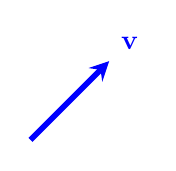
\begin{tikzpicture}
        %\draw[thin,gray!40] (-1,-1) grid (2,2);
        %\draw[<->] (-1,0)--(2,0) node[right]{$x$};
        %\draw[<->] (0,-1)--(0,2) node[above]{$y$};
        \draw[line width=2pt,blue,-stealth](0,0)--(1,1) node[anchor=south west]{$\mathbf{v}$};
        \end{tikzpicture}
        \hspace*{3cm}
        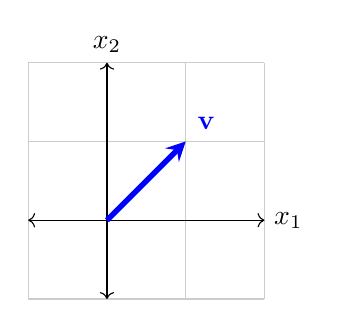
\begin{tikzpicture}
        \draw[thin,gray!40] (-1,-1) grid (2,2);
        \draw[<->] (-1,0)--(2,0) node[right]{$x_1$};
        \draw[<->] (0,-1)--(0,2) node[above]{$x_2$};
        \draw[line width=2pt,blue,-stealth](0,0)--(1,1) node[anchor=south west]{$\mathbf{v}$};
        \end{tikzpicture}
        \end{center}
\emph{Notice, even by placing $\mathbf{v}$ on paper, we have essentially chosen coordinates.} 

To see the transformation laws visually, we can place two vectors (left) and with coordinates (right).
        \begin{center}
        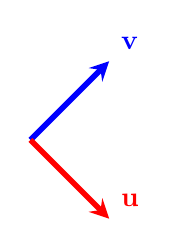
\begin{tikzpicture}
        %\draw[thin,gray!40] (-1,-1) grid (2,2);
        %\draw[<->] (-1,0)--(2,0) node[right]{$x$};
        %\draw[<->] (0,-1)--(0,2) node[above]{$y$};
        \draw[line width=2pt,blue,-stealth](0,0)--(1,1) node[anchor=south west]{$\mathbf{v}$};
        \draw[line width=2pt,red,-stealth](0,0)--(1,-1) node[anchor=south west]{$\mathbf{u}$};
        \end{tikzpicture}
        \hspace*{3cm}
        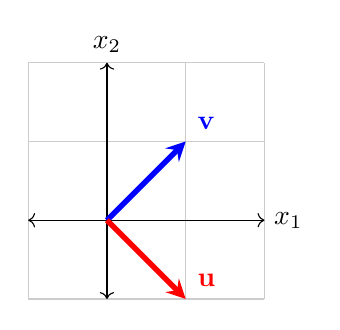
\begin{tikzpicture}
        \draw[thin,gray!40] (-1,-1) grid (2,2);
        \draw[<->] (-1,0)--(2,0) node[right]{$x_1$};
        \draw[<->] (0,-1)--(0,2) node[above]{$x_2$};
        \draw[line width=2pt,blue,-stealth](0,0)--(1,1) node[anchor=south west]{$\mathbf{v}$};
        \draw[line width=2pt,red,-stealth](0,0)--(1,-1) node[anchor=south west]{$\mathbf{u}$};
        \end{tikzpicture}
        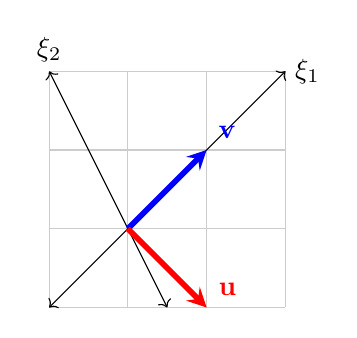
\begin{tikzpicture}
        \draw[thin,gray!40] (-1,-1) grid (2,2);
        \draw[<->] (-1,-1)--(2,2) node[right]{$\xi_1$};
        \draw[<->] (.5,-1)--(-1,2) node[above]{$\xi_2$};
        \draw[line width=2pt,blue,-stealth](0,0)--(1,1) node[anchor=south west]{$\mathbf{v}$};
        \draw[line width=2pt,red,-stealth](0,0)--(1,-1) node[anchor=south west]{$\mathbf{u}$};
        \end{tikzpicture}
        \end{center}
No matter the choice of coordinates, the ratio of lengths and angle between these vectors stays constant. Without going into more detail, this is a requirement for tensors in general.  

\section{Vector spaces}
Here we will take $(V,\field)$ to be a finite dimensional vector space of dimension $n$ over a field $\field$. When we can, we will work without choosing a basis since we have discusses the requirement of tensors to be independent of the choice of coordinates. Coordinates should not change the fundamental structure we care about.

It is possible to do most everything we do here over a module $(\mathcal{M},R)$ over a ring $R$, but this will not be important for now.  It is, however, important when we consider the case of tensor spaces on a smooth manifold $M$ since this will actually be a $C^\infty(M)$-module.

\subsection{Preliminaries and notation}

Let $\linmap$ denote a linear map between vector spaces.  Then, recall that given finite dimensional vector spaces $(V,\field)$, $(W,\field)$ of dimension $n$ and $m$ respectively, we have
\begin{itemize}
    \item $\Hom(V,W)\coloneqq \left\{f\colon V\linmap W\right\}$ is a vector space over $\field$, specifically of dimension $nm$;
    \item $\End(V)\coloneqq \Hom(V,V)$ is a vector space over $\field$ of dimension $n^2$;
    \item $\Aut(V)\coloneqq \left\{ f\colon V\linmap V ~\vert~ \textrm{$f$ is invertible}\right\}$;
    \item $V^*\coloneqq \Hom(V,\field)$;
    \item Finite dimensional vector spaces $(V,\field)$ and $(W,\field)$ are isomorphic if $\dim(V)=\dim(W)$.
    \begin{itemize}
        \item in finite dimensional vector spaces, $V\cong V^{**}$;
        \item in finite dimensional vector spaces, $\dim(V)=\dim(V^*)$;
        \item this does not hold in the infinite dimensional case. Take 
        \[V=L^1([0,1],\R) ~\implies~ V^*\cong L^\infty([0,1],\R)
        \]
        but
        \[
        V\ncong V^{**}\cong L^1_{\textrm{loc}}([0,1],\R).
        \]
    \end{itemize}
\end{itemize}

\section{Tensors}
There are a few ways of defining tensors.  All of them agree in the end, but I will take this approach.

\begin{definition}
A \emph{$(p,q)$-tensor} $T$ is a multilinear map
\[
T\colon \underbrace{V^*\times \cdots \times V^*}_{\textrm{$p$ copies}}\times \underbrace{V\times \cdots \times V}_{\textrm{$q$ copies}} \linmap \field.
\]
Here, multilinear just means that $T$ is linear in each input.
\end{definition}


\subsection{Tensor Spaces}
\begin{definition}
We define the space $T^p_q V$ of $(p,q)$-tensors on $V$ by writing
\[
\underbrace{V\otimes \cdots \otimes V}_{\textrm{$p$ copies}} \otimes \underbrace{V^*\otimes \cdots \otimes V^*}_{\textrm{$q$ copies}} \coloneqq \left\{ T ~\vert~ \textrm{$T$ is a $(p,q)-$tensor}\right\}.
\]
\begin{itemize}
    \item $T_q^pV$ is a vector space itself.
    \begin{itemize}
        \item For $T,S \in T_q^pV$, $T+S$ is defined pointwise and $T+S\in T_q^pV$.
        \item For $\lambda \in \field$ and $T\in \tspace$, we have that $\lambda T \in \tspace$.
    \end{itemize}
\end{itemize}
\end{definition}

It will help us to do an example with a chosen basis.  If we invoke a basis, I will choose the standard basis for both $V$ and $V^*$.  That is
\begin{itemize}
    \item $V$ has the basis $\{e_1,\dots,e_n\}$.
    \item $V^*$ has the \emph{dual basis} $\{e^1,\dots,e^n\}$ which satisfy $e^i(e_j)=\delta^i_j$.
\end{itemize}

\begin{example}[Basis and computation]
Let us fix $\dim(V)=2$ and $\field = \R$ and consider a tensor of the form
\[
G\colon V\times V \to \R.
\]
That is, $G\in T_2^0V$.  We have the canonical basis vectors $e_1,e_2$ for $V$ and dual basis vectors $e^1, e^2$ for $V^*$.  We can then construct a basis for the space
\[
T_2^0V \equiv V\otimes V
\]
by overusing the symbol $\otimes$ to create the basis vectors
\[
e^1\otimes e^1, ~e^1\otimes e^2,~ e^2\otimes e^1,~ e^2\otimes e^2.
\]
Then we can write any $G\in T_2^0V$ by a linear combination of the basis vectors by
\[
G\coloneqq \sum_{i=1}^2\sum_{j=1}^2 g_{ij}e^i\otimes e^j.
\]
Let us pause and make a few remarks.
\begin{itemize}
    \item When the basis for $V$ is understood, the basis for $V\otimes V$ is as well.  
    \item Given this, it suffices to understand just the coefficients $g_{ij}$ of the tensor $G$ much as we tend to just care about the coefficients of a matrix in linear algebra.
    \item In order to compactify notation, we adopt the \emph{Einstein summation convention} in that repeated indices are expected to be summed over. That is
    \[
    g_{ij}e^i\otimes e^j \equiv \sum_{i=1}^2 \sum_{j=1}^2 g_{ij}e^i \otimes e^j.
    \]
\end{itemize}
How do the vectors $e^i\otimes e^j$ act on the basis elements $e_k$ of $V$? We define
\[
e^i\otimes e^j (e_k,e_l)=e^i(e_k)\cdot e^j(e_l)=\delta^i_k\delta^j_l \in \field.
\]
Now, let us pick two vectors $u=u^ie_i$ and $v=v^ie_i$. Then, using the multilinearity of $G$, we have
\begin{align*}
G(u,v)&=g_{ij}e^i\otimes e^j(u^ke_k,v^le_l)\\
&= g_{11}e^1\otimes e^1(u^k e_k,v^l e_l)+g_{12}e^1\otimes e^2(u^k e_k,v^l e_l)+g_{21}e^2\otimes e^1(u^k e_k,v^l e_l) + g_22(u^k e_k,v^l e_l).
\end{align*}
Take, for example
\begin{align*}
    g_{11}e^1\otimes e^1 (u^k e_k,v^l e_l)&= g_{11}e^1\otimes e^1 ( u^1e_1 + u^2 e_2, v^1 e_1 + v^2 e_2)\\
    &=g_{11}e^1\otimes e^1(u^1 e_1, v^1 e_1) + g_{11}e^1\otimes e^1(u^1 e_1, v^2 e_2) \\
    &\qquad +g_{11}e^1\otimes e^1(u^2 e_2, v^1 e_1)+g_{11}e^1\otimes e^1(u^2 e_2, v^2 e_2)\\[5pt]
    &=g_{11}u^1v^1e^1\otimes e^1(e_1, e_1) + g_{11}u^1v^2e^1\otimes e^1(e_1,e_2) \\
    &\qquad +g_{11}u^2v^1e^1\otimes e^1(e_2, e_1)+g_{11}u^2v^2e^1\otimes e^1(e_2, e_2)\\[5pt]
    &= g_{11}u^1v^1\delta^1_1\delta^1_1 + g_{11}u^1v^2\delta^1_1\delta^1_2+g_{11}u^2v^1\delta^1_2\delta^1_1+g_{11}u^2v^2\delta^1_2\delta^1_2\\
    &= g_{11}u^1v^1.
\end{align*}
This is why the Einstein summation tool is so handy! Plus, we can now apply this to the whole tensor so that we find
\[
G(u,v)=g_{11}u^1v^1+g_{12}u^1v^2+g_{21}u^2v^1+g_{22}u^2v^2=g_{ij}u^iv^j.
\]
Some more remarks are in order.
\begin{itemize}
    \item We can understand the vectors and tensors just by the coefficients when the basis is assumed or not important.  This compactifies our notation quite a bit without really losing any valuable information.
    \item We can determine the \emph{compenents} of a given tensor $G$ by
    \[
    g_{ij}=G(e_i,e_j).
    \]
    This is an important fact.
\end{itemize}
\end{example}

\noindent \textbf{Warning:} We often drop the notation $g_{ij}e^i\otimes e^j$ and just refer to the components of the tensor $g_{ij}$.  However, not all objects with sub/superscripts are tensors!  Take for example, $\epsilon_{ijk}$ which is the Levi-Civita symbol or $\Gamma^i_{jk}$ which is the Christoffel symbol. The term ``symbol" is often used to emphasize the fact that these objects do not transform like tensors.

\begin{example}[Tensor Spaces]
Recall that we said tensor spaces are also vector spaces in their own right.  In some sense, we have already noticed this with the previous example, but let us be a bit more explicit. 

Let $T,S \in \tspace$ and $\lambda \in \field$.  Then we can define a new tensor $Q \in \tspace$ by
\[
Q=T+\lambda S.
\]
Then we can take $q$ vectors $v_1,\dots,v_q\in V$ and $p$ dual vectors $\omega_1,\dots,\omega_p\in V^*$ and define
\[
Q(\omega_1,\dots,\omega_p,v_1,\dots,v_q)\coloneqq T(\omega_1,\dots,\omega_p,v_1,\dots,v_q)+\lambda S(\omega_1,\dots,\omega_p,v_1,\dots,v_q).
\]
This extension makes $\tspace$ a vector space.
\end{example}

\begin{remark}
All of what we have done here can be generalized a bit.  For example, it is possible to consider tensor products of different vector spaces.  That is, we can take
\[
V\otimes W
\]
and make sense of this as a tensor of the form
\[
T\colon V^* \times W^* \to \field.
\]
This is not so hard to work through, and I will leave it to you. 
\end{remark}

\subsection{Tensor Product of Tensors}
We are tending to overload the symbol $\otimes$, and are here to do it again!  Now, we can consider the product of two tensors.  In doing this, we are making the tensor space into a graded algebra. 

\begin{definition}
The \emph{tensor product} of two tensors $T\in \tspace$ and $S\in T_s^rV$ is written as $T\otimes S$ and we have that $T\otimes S \in T_{q+s}^{p+r}V$. 

We then define
\[
T\otimes S(\omega_1,\dots,\omega_p,\omega_{p+1},\dots,\omega_{p+r},v_1,\dots,v_q,v_{q+1},\dots,v_{q+s})=a\in \field
\]
in the following way.  We take
\begin{align*}
a=T(\omega_1,\dots,\omega_p,v_1,\dots,v_q)\cdot S(\omega_{p+1},\dots,\omega_{p+r},v_{q+1},\dots,v_{q+s}). 
\end{align*}
\end{definition}

\subsection{Tensor Algebra}
The linear space $\tspace$ for some $(p,q)$ can be extended to an algebra by adopting the operation $\otimes$ as the multiplication in the algebra.  We write define the tensor algebra by
\[
\mathcal{T}(V) \coloneqq \bigoplus_{p,q\geq 0} \tspace.
\]
\textcolor{blue}{It seems like this gives us an algebra with two gradings.  One on the number of $V$ elements and the other on the number of $V^*$ elements.} 

\begin{example}
See that if we take $T\in \tspace$ and $S\in T_s^r V$ (i.e., $T,S \in \mathcal{T}(V)$) that we can take
\[
T\otimes S \in T_{q+s}^{p+r} \subset \mathcal{T}(V).
\]
\end{example}

\begin{example}
We can build up $\tspace$ using the tensor algebra.  Pick a basis $\{e_1,\dots,e_n\}$ for $V$ and let $\{e^1,\dots,e^n\}$ be the corresponding dual basis.  Then we can take
\begin{align*}
    T &= t_I^J e^I\otimes e_J\\
    S &= s_K^L e^K \otimes e_L
\end{align*}
where $I$, for example, represents the indices $i_1\dots i_q$ for $e^{i_1} \otimes \dots \otimes e^{i_q}$. 

Taking $p=q=r=s=1$ and $\dim(V)=2$, we can have
\begin{align}
    T &= t_i^j e^i \otimes e_j = t_1^1 e^1 \otimes e_1 + t_1^2 e^1 \otimes e_2 + t^2_1 e^1 \otimes e_2 + t_2^2 e^2 \otimes e_2\\ 
    S &= s_i^j e^i \otimes e_j = s_1^1 e^1 \otimes e_1 + s_1^2 e^1 \otimes e_2 + s^2_1 e^1 \otimes e_2 + s_2^2 e^2 \otimes e_2.
\end{align}
\textcolor{red}{whoops I used $s$ in two different ways.}

Then we take
\[
T\otimes S = (t_i^j e^i \otimes e_j)\otimes (s_k^l e^k \otimes e_l) = t_i^js_k^l e^i\otimes e^k \otimes e_j\otimes e_l. 
\]
We can write $T\otimes S = R$ and note that $r_{ik}^{jl}=t_i^js_k^l$ completely determines the product tensor when the basis is understood.  
\end{example}

\begin{question}
\textcolor{blue}{Is this saying that the tensor algebra is commutative? It shouldn't be since the matrix multiplication is not commutative!}
\end{question}

\subsection{Special Cases}
There are a few things we should do to reconcile the notion of tensors with objects we have seen before.  We will reuinite the tensor spaces $T_0^1V$ with $V$, $T_1^0V$ with $V^*$, and $T_1^1V$ with $\End(V)$. Keep in mind we are working over finite dimensional vector spaces and these may or may not hold in the case where $\dim(V)=\infty$!

\begin{proposition} 
We have that $T_0^1V\cong V$.
\end{proposition}
\begin{proof}
\[
T_0^1V = \left\{T\colon V^* \linmap \field\right\}.
\]
We take $v\in V$ and $f\in V^*$ and note that we can take
\[
v\colon V^* \linmap \field
\]
by forcing
\[
v(f)\coloneqq f(v).
\]
Really, what we are saying here is that $T_0^1V\cong V^{**}$ which, since we are in finite dimension, means we have $V\cong V^{**}$. So, $T_0^1V\cong V$.
\end{proof}

\begin{proposition}
We have that $T_1^0V\cong V^*$.
\end{proposition}
\begin{proof}
Follows again from the the fact that $V\cong V^{**}$.  More specifically, we have that $V^*\cong (V^*)^{**}$.
\end{proof}

\begin{proposition}
We have that $T_1^1V\cong \End(V^*)$.
\end{proposition}
\begin{proof}
Given a $T\in T_1^1V$, we can construct a $\tilde{T}\in \End(V^*)$ by
\begin{align*}
\tilde{T}\colon& V^* \linmap V^*\\
&\omega \mapsto T(\omega,\cdot)\in V^*.
\end{align*}
\end{proof}

\begin{corollary}
We also have that $T_1^1V\cong \End(V)$.
\end{corollary}
\begin{proof}
Follows from the fact that $\dim(V)=\dim(V^*)$.
\end{proof}

\begin{remark}
Noting that $T_1^1(V)\cong \End(V)$ we can identify the $(1,1)$-tensors with linear maps $V\linmap V$.  This means that elements of $T_1^1(V)$ can be represented by $n\times n$ matrices.
\end{remark}

\subsection{Symmetric Tensors}
One special case of tensors are the \emph{symmetric tensors}.  These tensors are defined below.

\begin{definition}
A tensor $T\in \tspace$ is \emph{symmetric} if 
\[
T(\omega_1,\dots ,\omega_p,v_1,\dots,v_q)=T(\omega_{\sigma(1)},\dots,\omega_{\sigma(p)},v_{\pi(1)},\dots,v_{\pi(q)})
\]
for any permutations $\sigma$ and $\pi$.
\end{definition}

\begin{example}[Inner Product]
Take $\field=\R$. Then the inner product is an example of a nondegenerate positive definite symmetric $(0,2)$-tensor.  Specifically, we have that $G\in T_2^0V$ is of the form
\[
G\colon V\times V \to \R
\]
and satisfies
\begin{itemize}
    \item $G(u,v)=G(v,u)$ for any $u,v\in V$;
    \item $G(v,v)>0$ for $v\in V$ with $v\neq 0$;
    \item $G(u,v)=0$ $\forall v \in V$ if and only if $u=0$.
\end{itemize}
We usually represent $G$ by the matrix $g_{ij}$ where $g_{ij}=g_{ji}$ and the eigenvalues are positive.
\end{example}

\begin{proposition}
If we equip $V$ with an inner product $G$, then we have a canonical isomorphism between $V$ and $V^*$ by the Reisz representation theorem. 
\end{proposition}

\begin{proof}
We take $v\in V$ and note that mapping $v\mapsto G(v,\cdot)\in V^*$ is a linear bijection.  
\end{proof}

\begin{remark}
This is often why tensors are referred to by their \emph{rank} as opposed to their \emph{valence}.  That is, a $(p,q)$-tensor $T$ is sometimes referred to as having valence $(p,q)$.  But, with an inner product, we would just say that $T$ has rank $p+q$. In other words, we can raise and lower indices of vectors and dual vectors without any trouble.
\end{remark}

\subsection{Alternating Tensors}
A special breed of tensors are known as the \emph{alternating tensors}. These are specifically useful in the realm of differential topology.  They are the characters that allow us to integrate volumes properly.  
\begin{definition}
An \emph{alternating $k$-tensor} is a $(0,k)$-tensor such that
\[
T(v_1,\dots,v_k)=\sign(\sigma)T(v_{\sigma(1)},\dots,v_{\sigma(k)})
\]
when $\sigma$ is an odd permutation. 
\end{definition}

Amazingly, we get many nice properties from this definition.  Here are a few.
\begin{itemize}
    \item If $v_i=v_j$ (or, really, if $v_i\in \textrm{span}\left(\{v_1,\dots,v_{i-1},v_{i+1},\dots,v_{k}\}\right)$) then
    \[
    T(v_1,\dots,v_k)=0.
    \]
    \item If we let $\dim(V)=n$, then all alternating $(n+1)$-tensors are the zero tensor.
\end{itemize}

\begin{definition}
We define the space of alternating $k$-tensors as a vector space that we denote by $\Lambda^k(V)$.
\end{definition}

There is a form of a tensor product that plays nicely with the alternating-ness of the tensors in $\Lambda^k(V)$.  

\begin{definition}
The \emph{wedge product} of an alternating $k$-tensor $\omega$ and an alternating $m$-tensor $\eta$ is written
\[
\omega \wedge \eta
\]
Without going into too much detail, just know that $\omega\wedge \eta \in \Lambda^{k+m}(V)$.
\end{definition}

\begin{remark}
This gives us a graded algebra 
\[
\Lambda(V)=\bigoplus_{i=0}^n \Lambda^i(V)
\]
known as the \emph{exterior (or Grassmann) algebra}.
\end{remark}

\begin{example}[Determinant]
Choose the standard basis for $V$, then given $v_1,\dots,v_n\in V$, we can compute the \emph{determinant} $\det(v_\bullet)\in \field$ (or signed volume) of these vectors by taking
\[
v_1\wedge \cdots \wedge v_n = \det(v_\bullet) (e_1\wedge e_2 \wedge \dots \wedge e_n)
\]
where $v_\bullet$ denotes the collection of vectors $\{v_1,\dots,v_n\}$.

Let's take the case of vectors in $\R^2$ given by $v_1=ae_1+be_2$ and $v_2=ce_1+de_2$ then
\begin{align*}
v_1\wedge v_2 &= (ae_1+be_2)\wedge (ce_1+de_2)\\
&= (ac)e_1\wedge e_1 + (ad)e_1\wedge e_2 + (bc)e_2\wedge e_1 + (bd)e_2\wedge e_2\\
&= (ad-bc)e_1\wedge e_2.
\end{align*}
Of course, this is exactly the determinant we have all seen for $2\times 2$-matrices. 
\end{example}

\begin{remark}
Can we see why this only allows us to define the determinant on square matrices?  If we took $n+1$ vectors (i.e., an $n\times (n+1)$-matrix) we will always receive 0.  If we took $n-1$ vectors (i.e., an $n\times (n-1)$-matrix) we will not have a unique value in the field to choose.
\end{remark}

\textcolor{blue}{Add in here the $e^1\wedge e^2$ eating vectors $v_1$ $v_2$ and spitting out volume.  Add in definition of wedge.}


\subsection{In the Case of Manifolds}
When we are dealing with a manifold $M$, the vector spaces we care about are the tangent space to $M$ at a point $p$ denoted $T_pM$ and its dual $T_p^*M$.  Elements $v\in T_pM$ are called \emph{tangent vectors} and elements $\omega \in T_p^*M$ are called \emph{covectors}.

If we attach more structure to $M$ by allowing a smoothly varying inner product (a nondegenerate symmetric positive definite $(0,2)$-tensor) $G$ on $T_pM$ at each point $p \in M$, we then call $M$ a \emph{Riemannian manifold} and call $G$ a $(0,2)$-tensor field.

Without the need for more structure on $M$, we can look at the calculus rules for integration on $M$ by investigating the forms.

\subsection{Exterior Algebra}

\begin{definition}
We denote the space of alternating $k$-tensor fields by $\Omega^k(M)$ by
\[
\Omega^k(M)\coloneqq \bigcup_{p\in M} \Lambda^k(T_p^*M).
\]
Then the \emph{exterior algebra of differential forms} is the algebra given by
\[
\bigoplus_{i=0}^n \Omega^i(M).
\]
\end{definition}
It turns out that we have an extra operation (other than $\wedge$) that works with the exterior algebra of differential forms.

\begin{definition}
The \emph{exterior derivative} is a map $d\colon \Omega^k(M)\linmap \Omega^{k+1}(M)$ that has the property $d\circ d =0$.  
\end{definition}

\subsection{de Rham Cohomology}
Now, letting $M$ be an $n$ dimensional manifold, we have built a structure that gives us a cochain complex.  Specifically, we have the \emph{de Rham complex}
\[
0\to \Omega^0(M)\dmap \Omega^1(M)\dmap \Omega^2(M)\dmap \dots \dmap \Omega^n(M)\dmap 0.
\]
Given $d \circ d=0$, we can now compute the cohomology of the de Rham complex. We call $k$ forms $\omega = d\alpha$ for some $\alpha$ a $(k-1)$-form \emph{exact} and $k$ forms $\eta$ such that $d\eta=0$ \emph{closed}.  We can then look at which forms are closed but not exact by investigating
\[
H_{dR}^k(M)\coloneqq \ker{d_{k}}/\mathrm{im} d_{k-1}.
\]

The salient fact here is that the de Rham cohomology is isomorphic to singular (or simplicial) cohomology with real coefficients.  

\section{Clifford Algebras}

\begin{itemize}
    \item Sources: \url{http://www.math.toronto.edu/mein/teaching/LieClifford/cl12.pdf}
\end{itemize}
Given the tensor subalgebra 
\[
\mathcal{T}^\bullet(V)\bigoplus_{m\geq 0} V^{\otimes m} \subset \mathcal{T}(V),
\]
we can consider other related structures.

If we equip $V$ with a (possibly degenerate) \emph{quadratic form} $Q \colon V \to \field$, then there is a natural quotient algebra generated.

\begin{definition}
We define the \emph{Clifford algebra} $\clifford$ to be 
\[
\clifford \coloneqq \bigslant{\bigoplus_{m\geq 0} V^{\otimes m}}{\langle v\otimes v - Q(v)1\rangle}
\]
where $I=\langle v\times v - Q(v)1\rangle$ is an  ideal generated by setting $v\otimes v$ equivalent to $Q(v)1 \in \field$. 
\end{definition}

Intuitively what this definition gives us is that we can collapse elements in the tensor subalgebra $\mathcal{T}^\bullet(V)$ to elements in the field $\field$. Specifically, we think of 
\[
v\otimes v \sim Q(v)1.
\]
So now we denote the multiplication in $\clifford$ (the \emph{Clifford product} by $\odot$ to distinguish this operation from the tensor product $\otimes$.  It also follows that \textcolor{blue}{we can create a swapping rule by looking at something like:}

\[
(u+v)\otimes (u+v) = Q(u+v)=u\otimes u + v \otimes u + u \otimes v + v\otimes v = Q(u)+Q(v) + u\otimes v + v\otimes u.
\]

\begin{example}
Let $\dim(V)=2$ and fix $Q\colon V \to \field$. Take
\begin{align*}
T&=t^{ij}e_i \otimes e_j\\
S&=s^{kl}e_k\otimes e_l.
\end{align*}
Then we can look at the equivalence class of $T\otimes S$ in the Clifford algebra.  That is, we take
\begin{align*}
T\odot S &= (t^{ij}s^{kl} e_i \otimes e_j \otimes e_k \otimes e_l) I.
\end{align*}
Now when we see any repeats $i=j$, $j=k$, or $k=l$ we can use the fact that
\[
e_i \otimes e_i \sim Q(e_i)1.
\]
So we find
\textcolor{blue}{Work this out and figure out how we can permute things to totally minimize this as far as possible. Whenever any two indices are equal we should be able to reduce.}
\end{example}


\end{document}